\documentclass{article}

% Language setting
% Replace `english' with e.g. `spanish' to change the document language
\usepackage[english]{babel}

% Set page size and margins
% Replace `letterpaper' with `a4paper' for UK/EU standard size
\usepackage[a4paper,top=2cm,bottom=2cm,left=3cm,right=3cm,marginparwidth=1.75cm]{geometry}

% Useful packages
\usepackage{amsmath}
\usepackage{graphicx}
\usepackage[colorlinks=true, allcolors=blue]{hyperref}
\usepackage{tikz}




\title{SIF3004 Final Year Project Proposal : RAdio Galaxy Environment Reference Survey (RAGERS) Project }
\author{Lim Ming Kang U2004991/1}

\begin{document}
\maketitle
\section{Problem Statement}

At the cosmological redshift of $2 < z < 3$ (observing the condition about 10.9 bllion years ago), the star forming rates (SFRs) is the highest, known as "the cosmic noon"\cite{Schreiber2020}.
Those galaxies are usually "dusty", enriched with dust which serves as the materials to star forming.
\medskip

\noindent A comprehensive understanding of those galaxies are important in understanding galaxies formation and evaluation of the early universe.\cite{Geach2016}


\paragraph{Characterisation} of the aforementioned galaxy overdensities with redshift, and the effect of Active Galatic Neuclei (AGN) activity on the growth of the central overdensities are to this day still not thorough.\cite{Ragers2021}
\medskip

\noindent Due to dust, those galaxies are not feasible to be observed in visible region, a telescope capable in observing in far infrared wavelength is needed to detect the galaxies.
\medskip

\noindent Data directly from telescope is not suitable for analysis, as noise and false detections may be presence, extensive data reduction and cleaning are essential to obtain a clean map for analysis. 
\medskip

\noindent The addition of far infrared data adds values to multiwavelength analysis, especially in obtaining photometric redshift.

\section{Objectives}
\begin{enumerate}
    \item To reduce data from raw telescope data to obtain analysable data (eg. source count) for a single source field
    \item To study statistically (eg. surface number density) of overdensities within a source field
    \item To obtain photometric redshift for detected submm galaxies in a source field.
\end{enumerate}
\section{Background}

\paragraph{Submillimetre Galaxies (SMGs)} are rare galaxies with high star formation rates $(>100M_\odot yr^{-1})$ \cite{DaCunha2021} populated in high redshift region. Suspected to be the progenitors for local giant galaxies, SMGs are good candidates to study the evolution of galaxies in high redshift. One challenge in observing SMGs is the amount of dust, that serves as the building blocks for star formation, which obscure visible light. However, far infrared/radio frequency are transparent to dust, thus the observation is allowed with submillimetre telecope. 

\paragraph{Overdensities} are regions in space where the density of matter is relatively higher than others. Events such as mergers of galaxies and active galatic nuclei (AGN) happen in overdensities region. At $z>1$, High redshift radio galaxies (HzRG) are usually in the region of overdensities where SMGs are. The dynamic between SMGs and HzRGs can be studied so have a more robust understanding of galaxy evolution at high redshift.

\paragraph{Telescope} operating at submillimetre region can be used to observe SMGs. An example is Atacama Large Millimeter Array (ALMA) telesope located in northern Chile, it operates at around wavelength $ 0.4mm < \lambda < 2.73mm$. Other examples are Fred Young Submillimeter Telescope operating at $\lambda=0.35mm$ and SCUBA-2 at James Clerk Maxwell Telescope (JCMT) operating at $\lambda=0.45mm$ and $\lambda=0.85mm$, whose data is used in the research of this proposal. Telescopes are usually associate with their proprietery software for data handling. For instances, CASA for ALMA, Starlink for JCMT and AIPS for Very Large Baseline Array (VLBA). They are extremely important to produce useful science data from noisy telescope data. Figure \ref{fig:reducevsunreduce} shows an example of the comparison between raw telescope data (up), and image after data reduction (down) 

\section{Research Methodology}

The research will be carried out on handling raw 0.85mm and 0.45mm data collected from JCMT SCUBA-2 under RAGERS Project, in collaboration with RAGERS Malaysia Team (from where the raw data is acquired). Data Reduction is run on Starlink software. The process of data handling is shown in Figure \ref{fig:flowchart1}

\paragraph{James Clerk Maxwell Telescope (JCMT)} is a 15m telesope designed to run on submillimetre wavelength (far infrared region). It is positioned at Maunakea, Hawaii.

\paragraph{SCUBA-2} is a camera attached on JCMT to observe at 450$\mu m$ and 850$\mu m$ (~666GHz and 353GHz) The data is formatted and stored in .sdf format, which is readable by starlink software.

\paragraph{The RAdio Galaxy Environment Reference Survey} is a JCMT program to observe overdensities of dusty galaxies within the Mpc region of 33 radio galaxies at redshift range $1 < z < 3.5$ and mass range $M\ast >=1010.8M\odot $ 

\paragraph{Source field} is a region spanning across few Mpc centered around a HzRG, which is located at $1 < z < 3.5$ 

\paragraph{Starlink} is a software consisting of several packages used to reduce and analyse data recorded by SCUBA-2 telescope, including (but not limited to) SMURF for data reduction and GAIA for data visualisation.

\begin{figure}
    \centering
    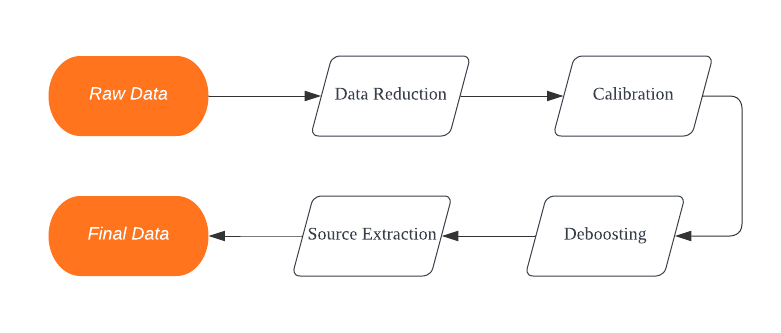
\includegraphics[width=100mm]{Flowchart.png}
    \caption{General process of preparing useful data from raw telescope data}
    \label{fig:flowchart1}
\end{figure}

\begin{figure}
    \centering
    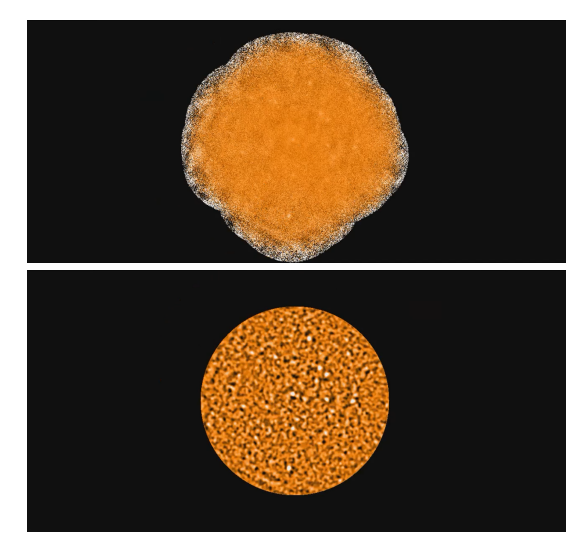
\includegraphics[width=100mm]{reducevsunreduce.png}
    \caption{An example of the comparison between raw telescope data (up), and image after data reduction (down)}
    \label{fig:reducevsunreduce}
\end{figure}

\begin{figure}
    \centering
    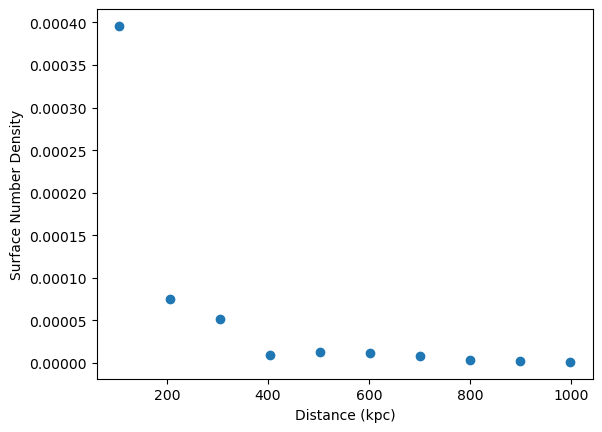
\includegraphics[width=100mm]{SNDensity.png}
    \caption{Surface number density as the function of distance from cluster center}
    \label{fig:sndensity}
\end{figure}

\begin{figure}
    \centering
    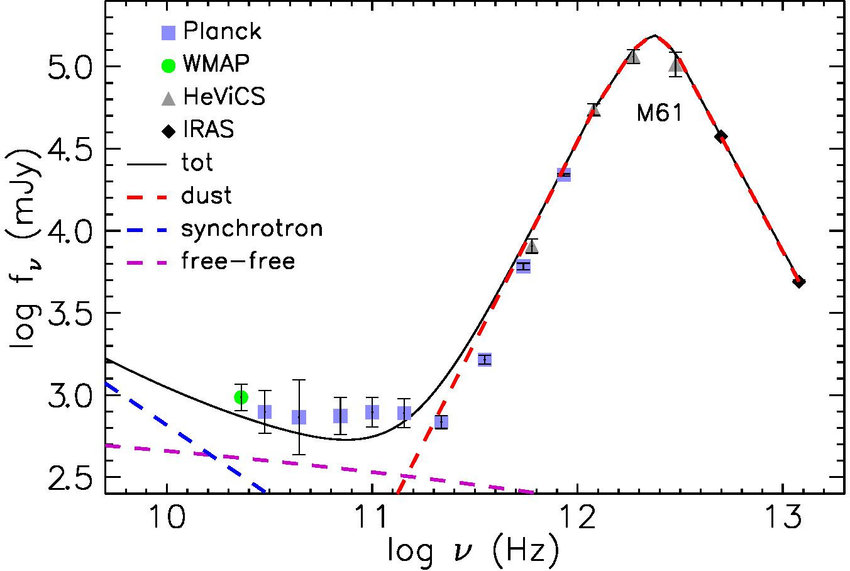
\includegraphics[width=100mm]{SED.png}
    \caption{An example of Spectral Energy Density graph, a logarithmic graph of flux density vs frequency}
    \label{fig:sedgraph}
\end{figure}

\section{Expected Results}
From the final reduced data, surface number density as the function of radius from center HzRG can be calculated from the number counts. Figure \ref{fig:sndensity} shows one example of graph of surface number density of cluster galaxies vs distance from a cluster center. A Spectral Energy Density (SED) of each detected submm galaxy can be calculated by combining multiwavelength flux density to obtain photometric redshift. An example of the stated graph is shown in figure \ref{fig:sedgraph}, from \cite{Zotti2018}

\section{Significance}
Surface number density is essential in studying the effect of environment. Photometric redshift is necessary to study the evolution of galaxies with redshift.

\bibliographystyle{plain}
\bibliography{sample}

\end{document}